%\newline

%Descripción general del módulo.
%Precondiciones necesarias.
%Por qué existe?
%Qué especificación tiene y cómo se maneja
%Comparación, como manejan los demás trabajos.

\chapter{Diseño}\label{cha:Diseño}

El objetivo principal de este capítulo es describir el diseño del framework propuesto para planificar tareas preemptive en sistemas embebidos heterogéneos. Se plantea la estructura del mismo junto con la descripción de su solución. 

Aunque se tomó como base el sistema embebido heterogéneo NVIDIA Jetson TX2, el diseño puede ser aplicado a cualquier dispositivo, siempre y cuando cumpla con la característica de tener memoria unificada, como la descrita en la sección \ref{sec:MemUni}.

\section{Descripción general del framework}

La solución propuesta se encuentra dentro de las siguientes clasificaciones:
\begin{itemize}

\item \textbf{Clasificación por implementación}: \textit{Basado en Software. Partición de Kernel.}
\item \textbf{Clasificación por planificación}: \textit{Planificación por prioridad.}
\item \textbf{Clasificación por modificación}: \textit{Modificación de código fuente.}



En la Figura \ref{fig:diagramabase} se muestra un diagrama de bloques sobre la arquitectura del framework propuesto. Cada uno de los bloques agrupa las bases necesarias para el funcionamiento del framework.
\newline

El framework está dividido en dos zonas de implementación, la primera tiene que ver con aquellas actividades que son propias con del Host, como lo es el protocolo de lanzamiento de los kernel (ver \ref{secc:lanzamientoKernel}. En el caso del manejo de la memoria, debido a que la tarjeta Jetson TX2 utiliza una arquitectura Pascal (ver \ref{secc:arqPas}), se cuenta con una memoria unificada con lo que se simplifican el manejo de las copias de memoria entre el en Host y el Device, resultando en que el módulo \textbf{Memoria} (ver \ref{secc:memoria}) pertenezca a ambas zonas, también se presenta el almacenamiento de los contextos de cada una de las tareas.

En la zona de implementación Device encontramos con el módulo \textbf{Puntos Preemptive} ver \ref{secc:puntosPreemptive}), como su nombre lo indica, se plantea la forma en que el framework implementa las suspensiones y reactivaciones de las tareas una vez alcanzado cada uno de los puntos. 

Un componente fundamental del framework es el módulo \textbf{Planificador} (ver \ref{secc:planificador}), ya que es en donde se dan las pautas para realizar la planificación de las tareas que se ejecutarán en un determinado momento en el Device. Pero para poder realizar dicha prioridad, se plantea el módulo \textbf{Asignación de prioridades} (ver \ref{secc:asigPrioridad}) el cual se encargará de seleccionar dentro de un conjunto de tareas aquella que tiene la mayor prioridad en un momento especifico de tiempo.

  \begin{figure}[ht]
      %\centering
     % \flushleft
        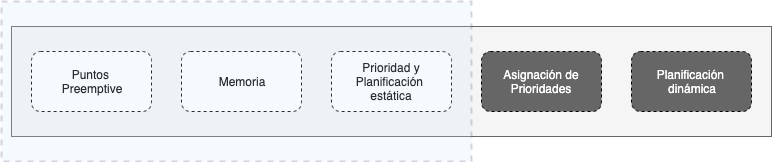
\includegraphics[scale=.6]{diagrama_framework}
        \caption{Diagrama del framework para la planificación de tareas preemptive en sistemas embebidos heterogéneos.}
        \label{fig:diagramabase}
    \end{figure}
  

  %Pero en el momento en el que se requiera tener un método de asignación de prioridades personalizado, es necesario tener un módulo que lo permita. Aunado a esto, si por alguna razón se solicita agregar tareas dinámicamente con el sistema en ejecución, se deben tener mecanismos para manejar cualquier interrupción o actualización de información del planificador. Ambos elementos son necesarios en un framework, pero sus componentes internos se dejarán para ser resueltos como trabajo futuro.
  
  %Clasficación y tipo de modificación.

Como se detallará más adelante, esta solución no es transparente al programador, es necesaria la modificación del código fuente, aunque en un inicio parecería que el rendimiento sería inferior al realizar comprobaciones continuas del estado del quantum, el modificar las bibliotecas del API de CUDA o el compilador del dispositivo ni tampoco la implementación de analizadores sintácticos para la lectura de directivas precompiladas está dentro de las posibilidades de acción del proyecto. 
Entonces s necesario modificar el código fuente, con esto también no debemos pensar en seleccionar los puntos más cercanos al óptimo para colocar directivas de precompilación.
\newline 


\end{itemize}   

  \begin{figure}[ht]
      \centering
     % \flushleft
        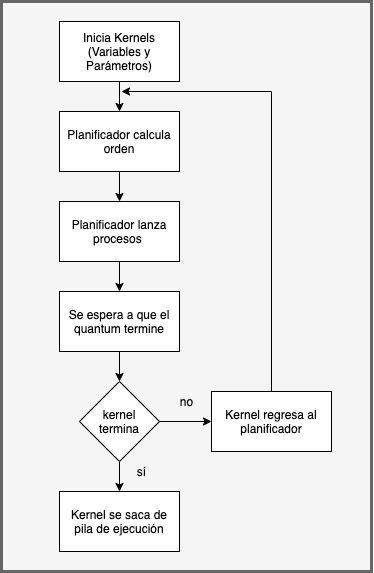
\includegraphics[scale=.6]{flujo}
        \caption{Diagrama del flujo del framework.}
        \label{fig:flujo}
    \end{figure}

\subsection{Precondiciones necesarias} \label{secc:precondiciones}
La precondición más importante es que el framework debe ser implementado en un programa que funciona correctamente, ya que se realizará una modificación en su código fuente para la implementación del modo preemptive.
No se permite la memoria dinámica ni compartida entre kernels.
No se permiten apuntadores complejos basados en objetos.
%No se permiten los GPU streams.
No se permite el llamado a funciones no rastreables.
El quantum de las tareas debe ser similar para que aquellas que estén en ejecución terminen en tiempos similares.

El número de threads por block debe ser menor o igual a la cantidad de threads disponibles en cada SM.

Los contextos de cada kernel deben poder coexistir en la memoria al mismo tiempo para que se puedan ejecutar y suspender en cada punto preempetive.

\section{Puntos preemptive}\label{secc:puntosPreemptive}

%Descripción general del módulo.

En una aplicación acelerada por el cómputo gráfico muchas veces se implementan más de una función kernel, y en el momento en que ejecutamos varias aplicaciones en el GPU habrá alguna que mantenga en sobretiempo los recursos causando así un retraso en la ejecución en general de todo el sistema.
\newline

Este módulo permite gestionar la actividad de un kernel a nivel de aplicación, aquí se marca la pauta el punto exacto donde se podrá realizar la administración del contexto de una tarea en ejecución, contará con tres casos principales, si se está iniciando el proceso, si está a la mitad de una ejecución o si ya ha terminado, con esto se podrá liberar las unidades de procesamiento para dar lugar a otras tareas de consumir recursos.
\newline

Se propone una serie de puntos de control que se incluirán explícitamente dentro del código que se desea implementar en modo preemptive, esto durante básicamente tres etapas iterativas del ciclo de vida de un kernel a)inicio, b)en ejecución y c)finalización. 
\newline

Este elemento tiene como objetivo que cada que se alcance alguno de los puntos de control dentro de un kernel y sea necesario detener su ejecución, se guarde una copia de su contexto actual en una estructura de datos para que cuando sea nuevamente su oportunidad de ejecución se reanude como si nunca se hubiera detenido. 
\newline

Una vez que una tarea, independientemente de en que momento de su ciclo de vida se encuentre seguirá ejecutándose en la GPU hasta que complete su cálculo o termine su quantum.
\newline

Al momento de lanzar la tarea siguiente en ejecución se inicializaran todas las variables necesarias en el nuevo contexto por medio de estructura copia de seguridad. Cuando se está en la etapa de inicio de un kernel, se inicializan tanto los datos necesarios para el funcionamiento de este en su cuerpo y en la estructura de datos.
\newline
%Qué especificación tiene y cómo se maneja?

Al inicio del algoritmo \ref{lst:declara} la función kernel está ligeramente modificada en sus parametros, ya que es necesario que reciba la estructura \textit{Backup} en donde se almacenará su contexto cuando se presente una suspensión preemptive, y se recibirá el apuntador al estado del quantum, dicho valor arrojará \textbf{\textit{true}} cuando se haya concluido el tiempo del quantum.
\newline

Como se mencionó anteriormente, esta solución es completamente basada en software, por lo que se debe modificar la función kernel, para mantener una convención que ayude a mitigar posibles problemas, todas las declaraciones de variables se deberán realizar en la primer fase, la cual se encuentra en las primeras lineas del kernel.
\newline

Las únicas declaraciones con inicialización permitidas en esta fase son aquellas que designan la posición tanto de los thread como de los blocks dentro de un grid, esto porque  su información es necesaria en cada una de las siguientes fases. La única variable que es necesaria para todos kernels es \textit{id\_block}, el que servirá para en las siguientes fases para extraer la información de la estructura \textit{Backup}.

\lstinputlisting[style=CStyle, frame=single,label=lst:declara,  basicstyle=\ttfamily\footnotesize, caption=Fase de declaración de variables.]{algorithms/fase_declaracion.c}

Enseguida pasamos a la fase de la inicialización de cada una de estas variables y como se muestra en el algoritmo \ref{lst:inicializa} nos apoyamos apoyándonos de una estructura \textit{switch-case} con tres casos dependiendo del estado de cada block. Para seleccionar cada uno de los casos debemos leer el valor que se encuentra en la estructura de copia de seguridad, esto por que hay que recordar que el kernel por si solo no sabe si es la primera vez que se ejecuta o es el producto de un cambio de contexto dentro del sistema.
\newline

Cada uno de estos tres diferentes estados es:

\begin{itemize}
\item \textit{\textbf{INICIO}}: Es el primer estado, y se presenta la primera vez que es lanzado un kernel, por lo que el valor inicial debe ser almacenado tanto en la variable local como en su espacio correspondiente en la estructura de copia de seguridad.

\item \textit{\textbf{EJECUCION}}: Este estado es el que se presenta una vez que ya se han inicializado las variables en el estado anterior, o cuando el planificador le da otra vez la oportunidad de ejecutarse para terminar el procesamiento. Aquí se copia la información de la estructura de copia de información a las variables locales, para trabajar con la información como si nunca se hubiera suspendido el kernel.

\item \textit{\textbf{TERMINADO}}: Debido a que muchas veces dentro de un kerel hay blocks que finalizan su procesamiento antes que otros, es necesario indicar que esa sección ya terminó y no requiere hacer ningún cálculo.
\end{itemize}

\lstinputlisting[style=CStyle, frame=single,label=lst:inicializa,  basicstyle=\ttfamily\footnotesize, caption=Fase de inicialización.]{algorithms/fase_inicializa.c}

Una vez inicializadas todas las variables podemos realizar el procesamiento objetivo del kernel. Para ello nuevamente preguntamos a la estructura de copia de seguridad el estado individual de cada block, dependiendo de lo que responda a cada uno, se realiza:

\begin{itemize}
\item \textit{\textbf{INICIO}}: Como se acaba de lanzar el kernel por primera vez, únicamente se cambia el estado del block a \textit{EJECUCION}, y como ahora se tiene un nuevo valor se puede ingresar al siguiente estado dentro del mismo switch.

\item \textit{\textbf{EJECUCION}}: Al entrar en este caso, en primera instancia se realiza el paso de procesamiento para resolver una parte del kernel original, esto se realiza dentro de una estructura \textit{do-while} para que al menos se realice una vez antes de que, o el quantum haya expirado, o se haya completado el procesamiento. Si algo de esto se cumple se rompe el ciclo y se pregunta si ya se completo el procesamiento, si es así, el estado del block en el backup se modifica a \textit{TERMINADO} y finaliza ese block sin realizar copia de seguridad para ahorrar tiempo de procesamiento.
En caso que no haya sido completado, significa que el quantum expiró, por lo que se deben guardar todas las variables locales en su correspondiente espacio designado dentro del backup, terminado esto, se finaliza el block.

\item \textit{\textbf{TERMINADO}}: En dado supuesto que se llegue a este caso, significa que se lanzó nuevamente el kernel por que existen blocks que aún no terminan su trabajo, con lo que este simplemente termina su ejecución.
\end{itemize}

\lstinputlisting[style=CStyle, frame=single,label=lst:procesamiento,  basicstyle=\ttfamily\footnotesize, caption=Fase de procesamiento.]{algorithms/fase_procesamiento.c}

\subsection{Condición de carrera}

La fase de procesamiento (ver algoritmo \ref{lst:procesamiento}) es un procedimiento en el que hay que poner especial atención ya que es donde se concentra el núcleo de las operaciones del kernel, aparte es donde se escriben variables compartidas por todo el grid, por ello hay que estar conscientes de que se debe evitar la condición de carrera.
\newline

Por ello en el \textit{case INICIO} únicamente el \textit{thread0} de cada block está habilitado para modificar el estado que se guarda en el \textit{backup}. Justo después del cambio de estado se debe esperar en una barrera para que todos los thread conozcan la actualización y no terminen abruptamente su procesamiento.
\newline

Lo anterior se repite en el \textit{case EJECUCION}, cuando se termina el procesamiento, nuevamente sólo el \textit{thread0} está autorizado para editar el contenido el arreglo \textit{estado} en la estructura de copia de estado.
\newline

Finalmente, si el procesamiento se realiza con ayuda de contadores, al momento de de que se expire el quantum, todos los threads deberán suspenderse cuando lleguen al mismo valor, por lo que lo más conveniente, en términos de memoria, es guardar sólo una copia de dicho contador. Entonces, una vez más el \textit{thread0} será quien almacene la información en su correspondiente lugar dentro de \textit{thread0}.

%%%%%%%%%%%%%%%%%%

  \section{Memoria}\label{secc:memoria}

  \subsection{Almacenamiento del contexto}
%Descripción general del módulo.

Es necesario la creación de una estructura de datos que guarde las copias de seguridad de los datos pertinentes que en conjunto formen el contexto de un kernel.
\newline

%Clasficación y tipo de modificación.



%Precondiciones necesarias.


%Por qué existe?



%Qué especificación tiene y cómo se maneja?

Todos los parámetros y variables que se encuentren dentro de una función kernel deben almacenarse en una una estructura, por lo que para cada uno de los kernel, se debe crear una estructura \textit{ad hoc}.
\newline

La estructura \textit{backup} (ver algoritmo \ref{lst:backupe}) almacena tres tipos de valores, primero todas aquellas variables locales necesarias para resolver el problema original del kernel. Debido a que estas variables son individuales por thread, debe guardarse una copia de cada thread de cada bloque. Está solución es muy costosa, por lo que se recomienda que la utilización de estas variables sea mínima o nula, en muchos casos podría almacenarse su contenido directamente en alguna de las variables \textit{resultado} que se pasaron como parámetro.
\newline

El segundo tipo de variables es el de tipo contador. Dependiendo del cálculo que se esté realizando, muchas veces se deberán paralelizar \textit{estructuras for} sin dependencia de datos, por esta razón, puede que después de un cierto número de iteraciones se pregunte por el estado del quantum, y en ese momento se realice la suspensión preemptive para todos los threads de un block. Como todos llegaron a ese punto, se puede simplemente guardar un valor del contador. En caso de que se esté utilizando contadores que son propiamente controlados por un punto de verificación de quantum, se deberá utilizar el formato de variable local.
\newline

Finalmente, debemos incluir un arreglo más que nos ayude a guardar el estado en que se quedó un block al ser detenido por el planificador.

\lstinputlisting[style=CStyle, frame=single,label=lst:backup,  basicstyle=\ttfamily\footnotesize, caption=Estructura Backup para almacenar el contexto.]{algorithms/backup.c}

  \subsection{Variables compartidas}
  
  Al momento de realizar una solución de GPGPU, se debe tener en cuenta que existirán variables que se deben mantener visibles tanto para el host como para el device. En el algoritmo \ref{lst:lanzamiento} de la sección \ref{secc:lanzamientoKernel} tenemos ciertas variables que deben ser compartidas entre ambos lados. 
    \newline
  
  Aparte de los parámetros que originalmente tiene la funcion kernel, se agregan dos más, una estructura \textit{backup} que almacena el contexto cuando se presenta una suspensión preemptive, y la bandera \textit{quantum\_expirado}, que nos indica si ya terminó el tiempo máximo de ejecución. Como estamos en el dominio de la memoria unificada, ambos parámetros existirán en la memoria global para que estén disponibles para ambos dispositivos.
  
  
  %%%%%%%%%%%%%%%%%%%%%%%%%%%%%%%%%%%%%%%%%%%%%%%%%%%%%%%%%%%%%

\section{Lanzamiento del kernel}\label{secc:lanzamientoKernel}

Dos precodiciones que plantea el framework (ver \ref{secc:precondiciones}) estrechamente relacionadas son que el framework planificará un número estático de kernels conocidos desde el inicio, y la segunda es que el código fuente esté disponible para su adecuación al sistema.
\newline

Cada una de las aplicaciones GPGPU que se ejecutarán en el sistema embebido deberán estar agrupadas en cabeceras de C. Al inicio de la ejecución del framework, se ejecutarán las aplicaciones de forma concurrente (Figura \ref{fig:appN_h}) para que todas alcancen el punto en que requieren realizar cálculos en la GPU.

  \begin{figure}[ht]
      \centering
     % \flushleft
        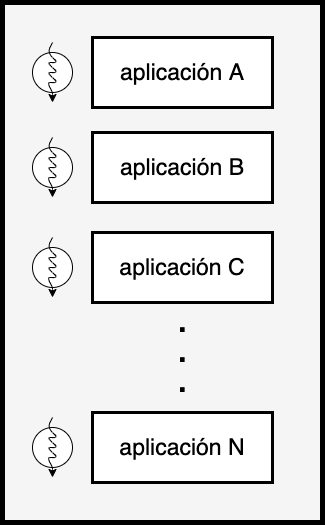
\includegraphics[scale=.3]{appN_h}
        \caption{Aplicaciones en ejecución concurrente.}
        \label{fig:appN_h}
    \end{figure}

Código de cada una de las aplicaciones se le debe añadir una serie de variables y parámetros para que el planificador pueda programar su ejecución. 
\newline

Se debe encapsular la llamada a la función kernel para que el planificador permita dar el orden de lanzamientos. Dentro de cada enclave se debe implementar una serie de variables y banderas para que el contexto pueda ser almacenado al alcanzar a cada punto preemptive. 
\newline

Es necesaria la definición de la estructura \textit{backup} especifica del kernel, también se debe indicar la duración del quantum con \textit{quantum\_time}, una bandera de control para verificar si ya ha expirado el quantum y una bandera que indicará si ya se ha ejecutado completamente el kernel. Finalmente, el planificador dará permiso de que se ejecute el kernel con la variable de control \textit{continuar\_eje}.

Ahora bien, una vez que se han definido las variables de control, se debe implementar un ciclo que terminará hasta que el kernel sea completado. Dentro debemos inicializar \textit{quantum\_expirado} en \textbf{\textit{false}} para indicar que se tiene tiempo de ejecución. La bandera \textit{continuar\_eje} será modificada por el planificador para permitir la ejecución del kernel. Una vez que sea planificado para su ejecución, se lanzará el kernel  y se esperará el tiempo definido para el quantum. Terminado este tiempo, se cambiará el estado de \textit{quantum\_expirado} a \textit{\textbf{true}} y se sincronizarán todos los threads del kernel con \textit{cudaDeviceSynchronize()} para cerciorarnos de que se terminó la ejecución del grid.
\newline

Ahora debemos cambiar el estado de \textit{continuar\_eje} a \textbf{\textit{false}} para que la tarea permanezca suspendida hasta que el planificador permita una nueva ejecución. Finalmente, se pregunta si todos los blocks completaron su trabajo.

\lstinputlisting[style=CStyle, frame=single,label=lst:lanzamiento,  basicstyle=\ttfamily\footnotesize, caption=Algoritmo para lanzamiento del kernel en el lado del host.]{algorithms/lanza_kernel.c}

Para poder determinar si un kernel ha terminado completamente su procesamiento, nos auxiliamos de la función \textit{kc} (Algoritmo \ref{lst:funcionkc}). Simplemente se pasa como parámetro el arreglo \textit{estado} de la estructura \textit{backup} y se pregunta si el estado de todos los blocks es \textit{\textbf{TERMINADO}}, de ser así, regresa \textbf{\textit{true}}.

\lstinputlisting[style=CStyle, frame=single,label=lst:funcionkc,  basicstyle=\ttfamily\footnotesize, caption=Función kernel completo.]{algorithms/funcion_kc.c}


\subsection{Planificador} \label{secc:planificador}

La GPU de la Jetson TX2 consta de dos SM con 128 cores cada uno\cite{SMJetson}.

Función Planificador

\lstinputlisting[style=CStyle, frame=single,label=lst:scheduler,  basicstyle=\ttfamily\footnotesize, caption=Función principal del planificador.]{algorithms/scheduler.c}
  
Función Ejecutar cola de Kernels

\lstinputlisting[style=CStyle, frame=single,label=lst:ejecutarKernels,  basicstyle=\ttfamily\footnotesize, caption=Función que ejecuta kernels encolados.]{algorithms/ejecutarKernels.c}

Función Busca kernels sin completar

\lstinputlisting[style=CStyle, frame=single,label=lst:kernelsSinCompletar,  basicstyle=\ttfamily\footnotesize, caption=Función busca kernels sin completar.]{algorithms/kernelsSinCompletar.c}

Estructura Task

\lstinputlisting[style=CStyle, frame=single,label=lst:Task,  basicstyle=\ttfamily\footnotesize, caption=Estructura task.]{algorithms/Task.c}
    	
\section{Asignación de prioridades} \label{secc:asigPrioridad}

La asignación de prioridades se realiza aplicando los algoritmos de tiempo real que se trataron en la sección \ref{sec:AlgoPlan}.

Función getTaskMayorPrioridad

\lstinputlisting[style=CStyle, frame=single,label=lst:getTaskMayorPrioridad,  basicstyle=\ttfamily\footnotesize, caption=Función que regresa la tarea con la mayor prioridad de un conjunto.]{algorithms/getTaskMayorPrioridad.c}

%%%%%%%%%%%%%%%%%%%%%%%%%%%%%%%%%%%%
\section{Resumen}




